\chapter{Problématique}
\label{chapter:problematique}

Dans ce chapitre, nous allons nous concentrer sur l'analyse d'applications web existantes. Cette dernière est importante, car elle nous permettra de définir les besoins clés d'une application de partage de \glspl{resinfo}. Cette étape correspond à la première phase de notre planning (cf. figure \ref{pic:ganttChart} en rouge). Vous pouvez considérer ce chapitre comme une introduction au chapitre \ref{chapter:analyseDesBesoins}, où nous développerons plus en détail les besoins spécifiques de \texttt{SourceCode}.

\section{Situation actuelle}
\label{section:situation}

Pour mieux comprendre l'univers des \glspl{resinfo}, nous avons analysé différentes plateformes. Bien que ces dernières n'apportent pas de solution précisément axée sur notre problématique, elles nous ont tout de même permis d'extraire des éléments pertinents à la création de notre plateforme : \texttt{SourceCode}.\\

Le tableau ci-dessous regroupe les différents sites web parcourus. Dans les sous-sections suivantes, nous listons les qualités et les défauts de chacune de ces plateformes. Vous retrouverez les captures d'écran représentant les différentes plateformes dans l'annexe \ref{annexe:problematique}.\\

\begin{table}[H]
    \centering
    \begin{tabular}{| l | l |}
    \hline
        Plateforme & Lien \\
    \hline
        Practice-it &
        \href{https://practiceit.cs.washington.edu/problem/list}{https://practiceit.cs.washington.edu/problem/list} \\ 
    \hline
        Hackerrank &
        \href{https://www.hackerrank.com/dashboard}{https://www.hackerrank.com/dashboard} \\ 
    \hline
        Leetcode &
        \href{https://leetcode.com/problemset/all/}{https://leetcode.com/problemset/all/} \\ 
    \hline
        Codeforces &
        \href{https://codeforces.com/problemset/}{https://codeforces.com/problemset/} \\ 
    \hline
        Codechef &
        \href{https://www.codechef.com/problems/challenge/}{https://www.codechef.com/problems/challenge/} \\ 
    \hline
        Coderbyte &
        \href{https://coderbyte.com/challenges/}{https://coderbyte.com/challenges/} \\ 
    \hline
    \end{tabular}
    \caption{Les différentes plateformes analysées}
    \label{table:compPlateforme}
\end{table}

Avant d'aller plus loin, nous tenons à mentionner l'outil \href{https://oer.uclouvain.be/}{OER UCLouvain} hors du champ de notre analyse. En effet, notre projet est une version simplifiée de leur application, car nous ne traitons qu'un seul domaine des \gls{oer} : les \glspl{resinfo}. Par conséquent, le système de recherche que le site propose ne correspond pas à la vision que nous avons pour notre type de plateforme étant donné qu'il est beaucoup plus complexe que ce que nous voulons mettre en place : Un catalogue de \glspl{resinfo}. Néanmoins, nous avons pu discuter avec \textit{Christine Jacqmot}, membre du \textit{Louvain Learning Lab}, afin de lui présenter notre projet et de voir comment se comporte l'outil \href{https://oer.uclouvain.be/}{OER UCLouvain} côté administration. Ses conseils nous ont aidés à améliorer notre prototype et dans le cas échéant, à rajouter dans le chapitre \ref{chapter:pourAllerPlusLoin} des précieuses pistes d'améliorations.
\pagebreak
\subsection*{Practice-it}

\href{https://practiceit.cs.washington.edu/problem/list}{Practice-it} est une plateforme permettant de résoudre des problèmes en Java en ligne. Comme le site le relate : \textit{la plupart des problèmes viennent des cours d'introduction en Java de l'université de Washington}.

\subsubsection*{Qualité(s)}

\begin{itemize}
    \item Les problèmes peuvent être résolus de manière interactive depuis la plateforme.
    \item La progression d'exercices résolus est sauvegardée.
    \item Les problèmes sont organisés sur plusieurs niveaux : par cours ou par l'année d'édition du livre contenant ces exercices -> Chapitres -> Thématiques -> Exercices.
    \item Accès à une recherche avancée par mots clés ou titre de recherche.
    \item Un exercice contient les informations suivantes :
    \begin{itemize}
        \item Titre
        \item Auteur
        \item Date de modification/création
        \item Langage de programmation
    \end{itemize}
\end{itemize}

\subsubsection*{Défaut(s)}

\begin{itemize}
    \item Interface très simpliste.
    \item \textbf{On doit se connecter} pour accéder à la recherche avancée.
    \item Pas de \gls{tagCat} pour la recherche avancée : les éléments sont affichés de manière pêle-mêle dans une liste déroulante conséquente.
    \item La recherche de problèmes sans la recherche avancée n'est pas pratique.
\end{itemize}

\subsection*{Hackerrank}

Cette plateforme a la volonté d'aider les développeurs à améliorer leurs compétences en programmation. Elle est aussi faite pour que les grandes entreprises puissent facilement trouver des développeurs ayant les compétences requises. Seule la partie "\textit{Practice}" du site est intéressante pour notre problématique.

\subsubsection*{Qualité(s)}

\begin{itemize}
    \item Le tableau de bord est séparé en plusieurs sections pratiques :
    \begin{itemize}
        \item Compétences de l'utilisateur
        \item Les différentes compétences proposées (langage de programmation, mathématiques,...)
        \item Tutoriel
    \end{itemize}
    \item Une barre de recherche est disponible pour trouver des exercices / challenges par leur titre.
    \item Lorsqu'on choisit un langage de programmation, l'interface de recherche présente trois catégories de \glspl{tag} :
    \begin{itemize}
        \item Statut (résolu ou non)
        \item Difficulté
        \item Sous-domaine (thématique)
    \end{itemize}
    \item Parmi les \glspl{tag}, on peut en sélectionner plusieurs dans la même catégorie (OU logique) tout en sélectionnant d'autres \glspl{tag} dans une autre catégorie (ET logique entre les différentes catégories).
    \item On peut résoudre de manière interactive le challenge depuis la plateforme (à condition d'être connecté).
    \item On peut noter le challenge sur 5 étoiles.
    \item Les tests cases et énoncés du challenge peuvent être téléchargés.
    \item Une section "\textit{Discussions}" est mise à disposition pour chaque challenge.
\end{itemize}

\subsubsection*{Défaut(s)}

\begin{itemize}
    \item Peu de catégories et de \glspl{tag} pour rechercher un challenge.
    \item Il faut obligatoirement se créer un compte pour suivre un tutoriel ou soumettre un challenge.
    \item La moyenne de note d'un challenge ne figure pas dans l'interface. On peut noter un exercice, mais on ne peut pas connaître "l'avis" général.
\end{itemize}

\subsection*{Leetcode}

Cette plateforme cherche à améliorer les compétences des développeurs en proposant des exercices et tutoriels sur des thématiques variées. Elle permet d'étendre ses connaissances en programmation en vue de préparer un prochain entretien avec une entreprise.

\subsubsection*{Qualité(s)}

\begin{itemize}
    \item Une barre de recherche est disponible pour trouver des exercices par leur titre, description ou identifiant (ID).
    \item Choix parmi différentes catégories :
    \begin{itemize}
        \item Algorithmes
        \item Base de données
        \item Terminal
        \item Concurrence
    \end{itemize}
    \item Deux grandes catégories de \glspl{tag} sont présentes :
    \begin{itemize}
        \item Topics
        \item Entreprises
    \end{itemize}
    \item Chacun des \glspl{tag} est associé à un nombre correspondant au nombre d'exercices contenant ce \gls{tag}.
    \item Possibilité de filtrer les exercices en fonction de la difficulté, du statut (résolu, à faire, essayé).
    \item On peut résoudre de manière interactive le challenge depuis la plateforme (à condition d'être connecté).
    \item On peut liker ou disliker un exercice.
    \item Une section "\textit{Discussions}" est mise à disposition pour chaque exercice.
    \item Chaque exercice peut se résoudre avec son langage de prédilection.
\end{itemize}

\subsubsection*{Défaut(s)}

\begin{itemize}
    \item Malgré un choix varié de \glspl{tag}, ces derniers ne sont pas classés dans des catégories différentes.
    \item Les \glspl{tag} ne sont pas directement accessibles depuis l'interface, car il faut scroller.
    \item Aucune spécificité au niveau des langages de programmation (exemple: des exercices en C pour la gestion de la mémoire).
    \item Il faut obligatoirement se connecter pour s'exercer avec la plateforme.
\end{itemize}

\subsection*{Codeforces}

CodeForces est une plateforme créée par une communauté de programmation axée sur la compétition et les concours.

\subsubsection*{Qualité(s)}

\begin{itemize}
    \item On peut voir le nombre d'utilisateurs ayant résolu le challenge.
\end{itemize}

\subsubsection*{Défaut(s)}

Cette plateforme est un exemple concret de site web que nous ne voulons pas créer tant l'ergonomie et les différentes fonctionnalités ne sont pas assez matures ou pertinentes à notre égard.\\

\begin{itemize}
    \item La recherche n'est pas claire du tout. Pour afficher la barre de recherche, il faut cliquer sur une flèche bleue (pas logique).
    \item On peut filtrer les challenges en cliquant sur un des \glspl{tag} présents sur un des exercices, mais on ne peut pas y rajouter un autre \gls{tag} (cela efface la précédente sélection).
    \item Possibilité de rajouter des \glspl{tag} avec un panneau latéral (sur la droite), mais les options sont très sommaires (difficultés, \glspl{tag} dans une liste déroulante conséquente). C'est aussi le seul moyen de prendre connaissance avec la panoplie de \glspl{tag} proposés.
    \item On peut filtrer les exercices par niveau de difficulté, mais il n'y a aucune indication pour nous dire ce que cela représente. Concrètement, il faut entrer un nombre entre plancher X et plafond Y (le plus grand nombre enregistré pour identifier la difficulté d'un exercice était de 3800).
    \item Aucun moyen de réinitialiser la recherche. La seule manière est de retirer manuellement les \glspl{tag} sélectionnés et le titre de recherche.
\end{itemize}

\subsection*{Codechef}

\textit{CodeChef} est un site de programmation compétitif. Il s'agit d'une initiative éducative à but non lucratif de Directi, qui vise à fournir une plateforme pour les étudiants, les jeunes professionnels du logiciel, afin qu'ils puissent s'exercer et affiner leurs compétences en programmation grâce à des concours en ligne. En outre, le programme "CodeChef For Schools" vise à atteindre les jeunes étudiants et à inculquer une culture de la programmation dans les écoles indiennes. (texte tiré de \href{https://en.wikipedia.org/wiki/CodeChef}{Wikipedia})


\subsubsection*{Qualité(s)}

\begin{itemize}
    \item La recherche est basée sur le niveau de difficulté : débutant, facile, normal, difficile et challenge.
    \item On interagir de manière interactive avec la plateforme pour soumettre son code.
    \item On peut filtrer des exercices par \glspl{tag} en utilisant une interface dédiée.
    \item On peut connaître le nombre d'exercices se rapportant à un \gls{tag}.
    \item Possibilité de filtrer par auteur.
\end{itemize}

\subsubsection*{Défaut(s)}

\begin{itemize}
    \item Il faut obligatoirement se connecter pour soumettre un exercice.
    \item Il n'y a pas de catégorie de \glspl{tag}, ils sont tous affichés de manière pêle-mêle depuis l'interface.
    \item Pas de barre de recherche pour trouver un exercice en fonction de son titre.
\end{itemize}

\subsection*{Coderbyte}

\textit{CoderByte} est une plateforme proposant divers challenges de programmation en vue d'améliorer les compétences des développeurs et les préparer à une future interview avec une entreprise.

\subsubsection*{Qualité(s)}

\begin{itemize}
    \item La plateforme propose un système de \glspl{tag} avec 3 catégories : difficulté, entreprise, \glspl{tag}. Il se situe dans un panneau latéral accessible sur le côté droit de l'écran.
    \item Parmi les \glspl{tag}, on peut en sélectionner plusieurs dans la même catégorie (OU logique) tout en sélectionnant d'autres \glspl{tag} dans une autre catégorie (ET logique entre les différentes catégories).
    \item On peut résoudre les challenges directement depuis la plateforme et sélectionner son langage de prédilection.
    \item Pas besoin de se connecter pour résoudre un challenge.
    \item On peut participer à une discussion autour d'un challenge particulier.
\end{itemize}

\subsubsection*{Défaut(s)}

\begin{itemize}
    \item Pas de barre de recherche pour trouver un exercice en fonction de son titre.
    \item Classification sommaire des \glspl{tag} (les langages de programmation sont mélangés avec les thématiques,...).
\end{itemize}

\subsection*{Conclusion sur l'analyse}

Cette analyse nous a permis de partir sur de bonnes bases pour la création de notre application web. Nous voulions nous inspirer de certaines interfaces proposant de bonnes idées au niveau de la recherche pure, car cette dernière sera l'une des fonctionnalités principales de \texttt{SourceCode}. \\

Certaines fonctionnalités comme l'espace de discussion sur un challenge spécifique ou encore la soumission de sa solution directement sur la plateforme demeurent de bonnes idées, mais pas nécessaires à l'élaboration d'une application comme \texttt{SourceCode}, car l'objectif premier est le référencement de \glspl{resinfo} avant tout. Dans une perspective future, l'intégration de ce genre de fonctionnalités pourrait bien sûr être envisageable, ce qui rendrait ce projet encore plus flexible.\\

Avec le support de cette analyse, nous avons pu constituer une liste des éléments importants devant être intégrés au projet. Cela a aussi servi à mettre sur papier nos idées à travers un patchwork que vous pourrez consulter dans la section \ref{section:problem}.


\section{Problème}
\label{section:problem}

Compte tenu de l'analyse des plateformes précédentes, nous allons nous intéresser aux obstacles à franchir pour créer une plateforme de partage de \glspl{resinfo}, en particulier la nôtre.\\

La recherche de \glspl{resinfo} demeure la base de \texttt{SourceCode}. Par conséquent, l'élaboration d'une \textbf{bibliothèque} proposant une recherche efficace et pratique est un premier jalon à traverser. Il faut que l'utilisateur comprenne assez rapidement comment interagir avec l'interface pour trouver des \glspl{resinfo} correspondant à ses critères de recherche (exemples : exercices avec le langage C, thématique sur les pointeurs,...).\\

Se pose ensuite la question du \textbf{contenu d'une \gls{fiche}}. Cette dernière contiendrait probablement un titre et une description (énoncé d'un exercice, tutoriel), mais le plus important reste son \textbf{référencement} à travers l'application. Il s'agirait alors d'intégrer un système de \glspl{tag} cohérent permettant de retrouver rapidement une \gls{fiche} dans la bibliothèque.\\

\textbf{Le système de \glspl{tag}} serait incontestablement le cœur de l'interface de recherche de \glspl{resinfo}. Non seulement il devrait être facilement accessible dans l'interface (ergonomie), mais il devrait aussi proposer une \textit{taxonomie} compréhensible par les utilisateurs de la plateforme. Nous entendons par \textit{taxonomie}, une catégorisation des différents \glspl{tag} pour faciliter la recherche (exemples : difficulté, cours, langage ...).\\

Pour qu'une application de cette envergure soit facilement maintenable en termes de contenu, un autre besoin à satisfaire serait la création d'une \textbf{interface de gestion} permettant d'ajouter des ressources, de créer des \glspl{tag} ... Sans cette interface, l'intérêt de la plateforme serait moindre, car l'ajout de ressources serait rendu difficile, voire impossible à réaliser pour le grand public.\\

Étant donné qu'une multitude d'utilisateurs ajouteraient du contenu sur la plateforme, un système de \textbf{modération} semble important à mettre en place. Dans cette perspective, il est alors question de déterminer une organisation sous \textit{différents types d'utilisateurs} avec des privilèges propres (simple visiteur, utilisateur avec un compte, administrateur). Sans cette modération, la plateforme ne pourrait pas prétendre à du contenu de qualité, car tout type de ressource serait alors publié dans la bibliothèque.\\

Pour poursuivre avec le critère de \textit{qualité} du contenu, il serait judicieux d'élaborer un \textbf{système de statuts} pour les ressources publiées. Les ressources validées seraient ainsi visibles dans la bibliothèque (accessible à tout public) tandis que les autres (non valides, en attente,...) seraient uniquement visibles depuis les interfaces de gestion. Reste à déterminer le nombre de statuts et leur utilité.\\

Toujours dans l'optique d'améliorer la qualité du contenu de la plateforme, un \textbf{système de vote} devrait être mis en place afin de laisser la communauté s'exprimer sur la pertinence d'une \gls{resinfo}. La modération est une première instance de validation des \glspl{resinfo} ajoutées sur la plateforme, mais nous estimons que la communauté doit aussi pouvoir donner son avis. Cela permettrait d'une part au créateur de la \gls{resinfo} d'améliorer sa \gls{fiche} et d'autre part aux administrateurs d'émettre une nouvelle évaluation de la \gls{resinfo}.\\

Afin de vous donner une petite idée de ce que nous avons imaginé après la première analyse des plateformes, nous vous proposons quelques illustrations de notre patchwork pour la partie bibliothèque et la consultation d'une \gls{fiche}. \textbf{Ceci n'est pas un design final de \texttt{SourceCode}}, mais plutôt une mise sur papier de notre conception de l'application web au vu des critères exposés précédemment.\\

\begin{figure}[H]
    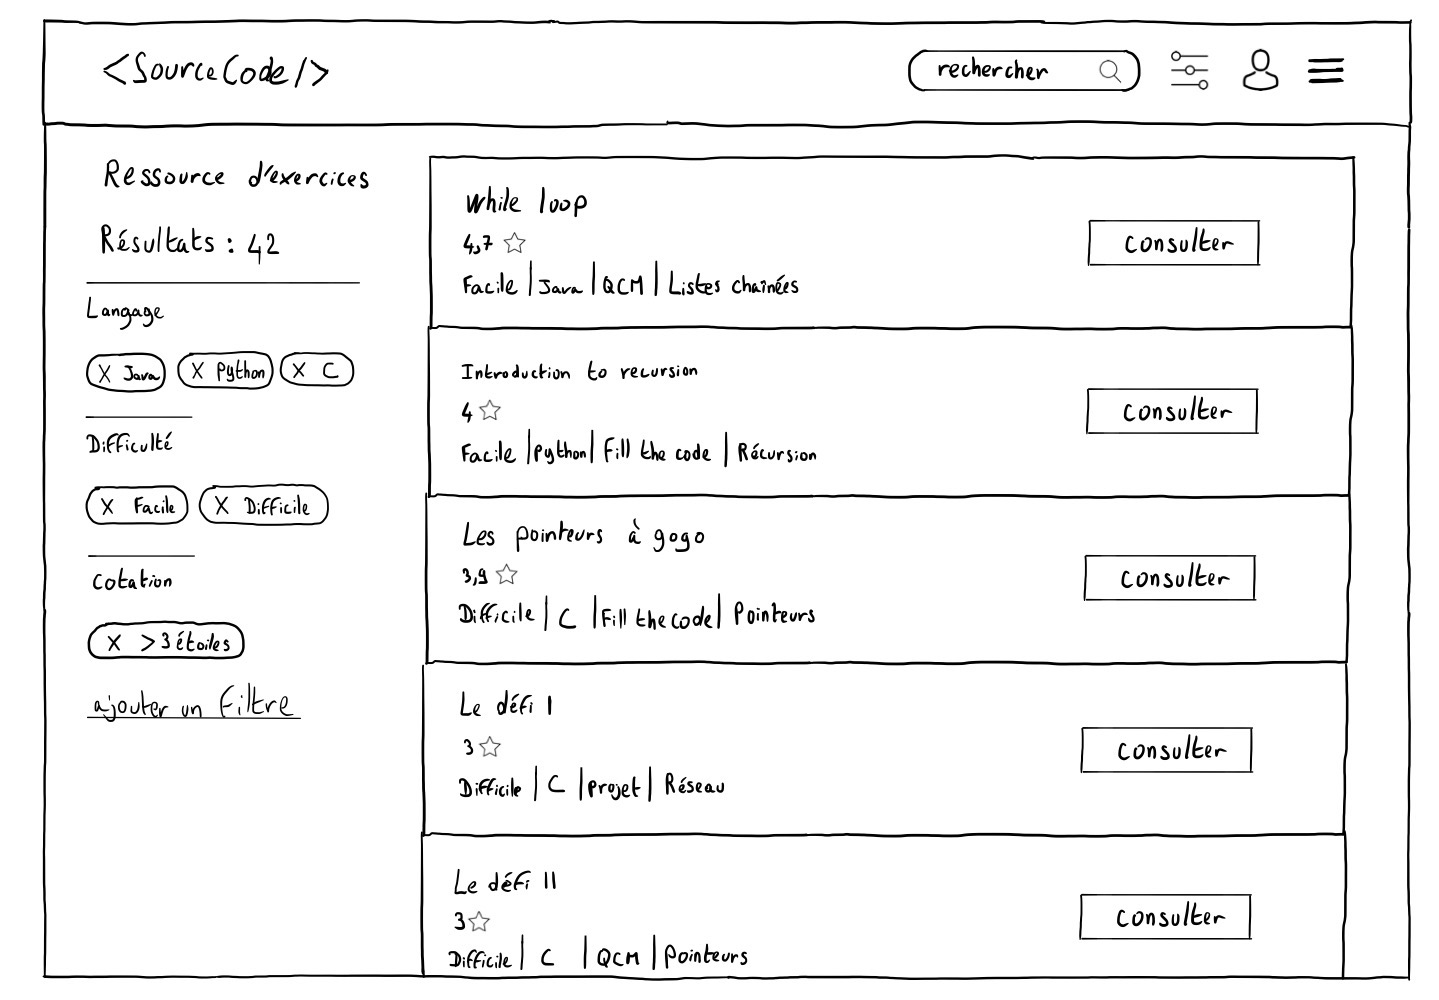
\includegraphics[width=\textwidth,height=\textheight,keepaspectratio]{images/library.JPG}
    \centering
    \caption{La page Bibliothèque}
\end{figure}
\label{figure:patchwork}

\begin{figure}[H]
    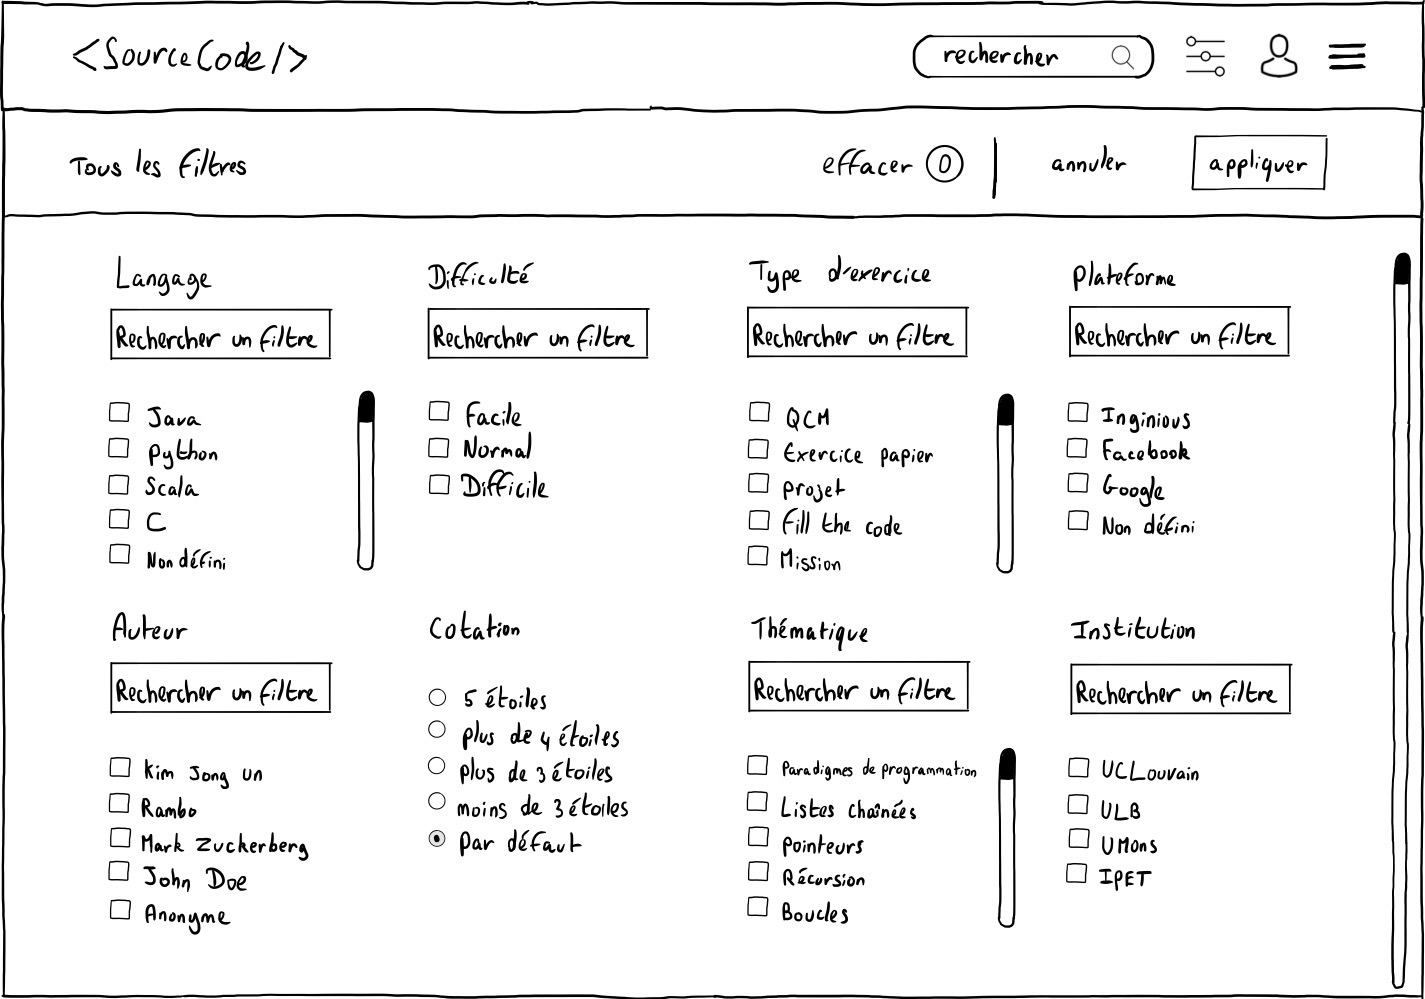
\includegraphics[width=\textwidth,height=0.45\textheight,keepaspectratio]{images/filters.JPG}
    \centering
    \caption{Représentation du système de filtres avec les \glspl{tag}}
\end{figure}
\label{figure:systemeDeFiltres}


\begin{figure}[H]
    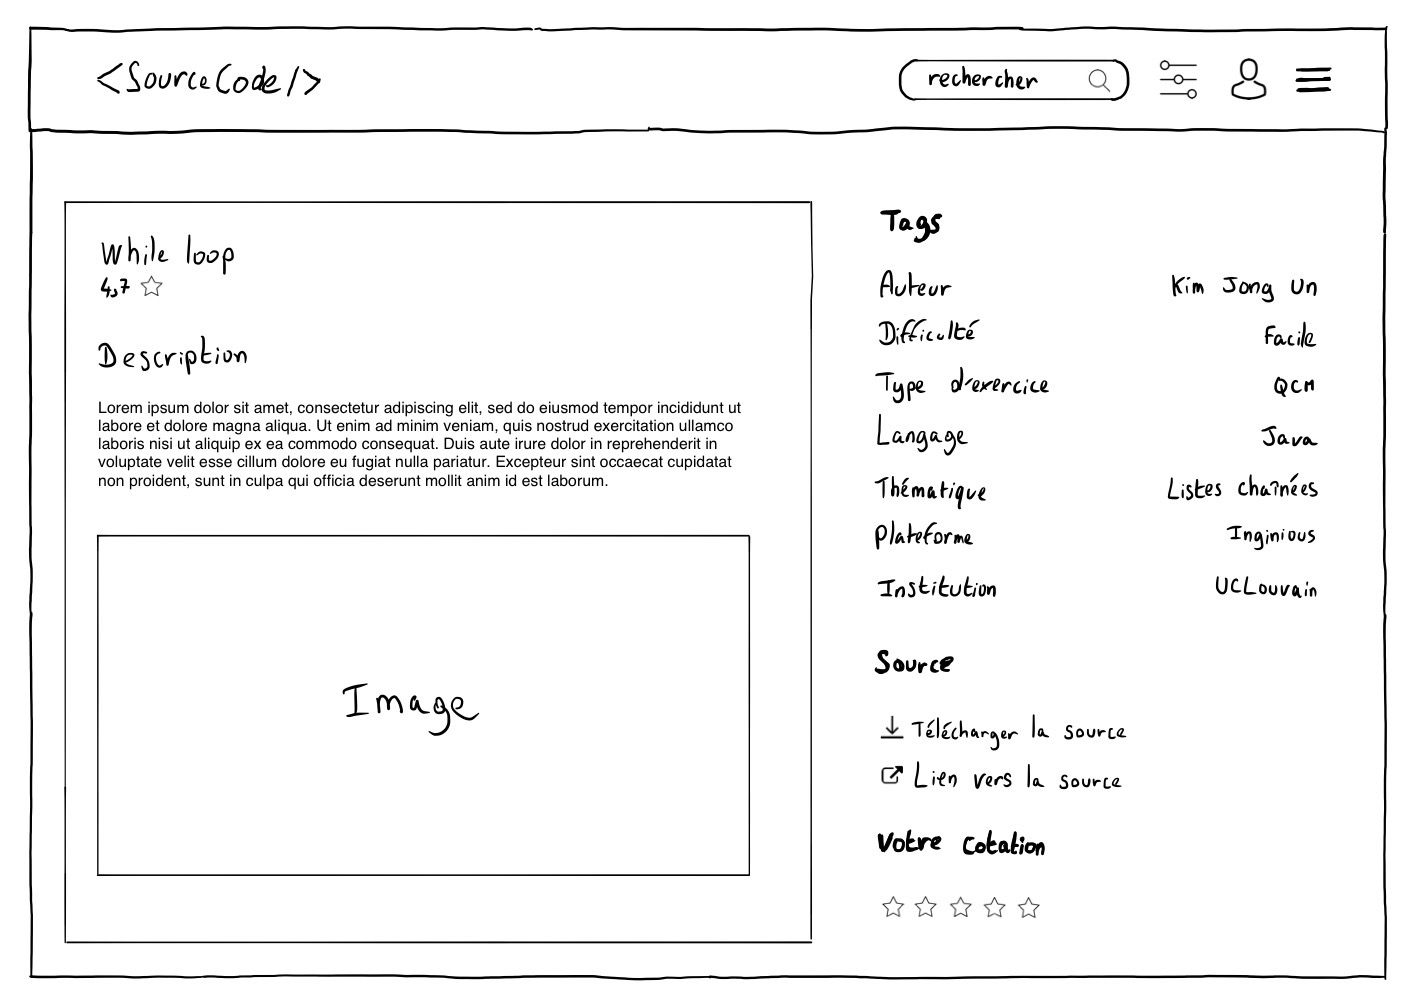
\includegraphics[width=\textwidth,height=0.45\textheight,keepaspectratio]{images/resource.JPG}
    \centering
    \caption{Page d'une \gls{fiche}}
\end{figure}

\pagebreak
\section{Défis à relever}
\label{section:challengesToDefeat}

Après avoir formalisé les besoins d'une application de partage de \glspl{resinfo}, nous allons maintenant lister ce que nous allons mettre en place pour réaliser notre plateforme. Notez que cette liste est introductive à l'analyse fonctionnelle relatée dans la section \ref{section:analyseFonctionnelle}, mais nous avions besoin de cette étape pour avoir une vue au global de \texttt{SourceCode} avant d'aller un peu plus dans les détails.

\begin{itemize}
    \item Proposer une interface simple et ergonomique à destination d'un public varié. Pour rappel, la cible principale est l'équipe pédagogique (professeurs, doctorants, formateurs,...), le reste étant majoritairement des étudiants. Peu importe le type d'utilisateur, l'outil doit être suffisamment clair que pour comprendre les fonctionnalités clés de l'application (recherche de \glspl{resinfo}, création de \glspl{fiche}, gestion des favoris ...).
    \item Créer un système de \glspl{tag} évolutif et extensible. Nous entendons par là la possibilité de créer/modifier/proposer des \glspl{tag}, créer/modifier des \glspl{tagCat},... . Cela permettra ainsi de ne pas figer l'application sur une poignée de \glspl{tag}, mais aussi de s'adapter à de nouvelles conventions en renommant certains d'entre eux.
    \item Proposer une interface de modération complète pour gérer les \glspl{tag}, les \glspl{tagCat}, les \glspl{resinfo} et les utilisateurs. En outre, les interfaces d'administration ne seraient disponibles qu'à partir du moment où l'utilisateur possède un compte éligible d'administrateur. Les autres interfaces de gestion pour ses propres \glspl{resinfo} devraient être accessibles aux utilisateurs possédant un simple compte utilisateur.
    \item La recherche de \glspl{resinfo} doit fonctionner de manière efficace. À ce propos, le site \textit{coderByte} propose une bonne façon de rechercher des exercices, avec un panneau latéral comportant des \glspl{tag} rangés dans des catégories. Nous allons donc nous inspirer de cette pratique pour naviguer dans la bibliothèque, tout en ajoutant une barre de recherche pour naviguer dans les titres des \glspl{resinfo}.
    \item Créer et intégrer à l'application un outil pour importer/exporter rapidement des \glspl{resinfo}, des \glspl{tag} et \glspl{tagCat}. Ajouter des \glspl{resinfo} peut être chronophage dans le cas où il y aurait quelques dizaines de \glspl{fiche} à créer depuis l'interface de gestion. Nous souhaitons donc automatiser le processus de création en proposant un format d'import acceptant les éléments précédemment cités. À l'inverse, exporter des \glspl{resinfo} depuis notre plateforme devrait être rendu possible afin de partager les ressources avec d'autres plateformes par exemple.
    \item Une piste non explorée par les différentes plateformes précédemment analysées est de proposer une recherche de \glspl{resinfo} plus attractive. Nous pensons donc à intégrer un historique et un système de favoris pour naviguer plus aisément dans les recherches effectuées antérieurement.
\end{itemize}

\pagebreak
Pour conclure ce chapitre et cette section, il est important de noter que la création d'une application web à destination d'un public varié demande un investissement conséquent en termes de temps. Il s'agit de créer une interface satisfaisant les attentes de chaque groupe d'utilisateurs tout en proposant un projet maintenable et évolutif pouvant satisfaire les besoins futurs.\\

Chaque page doit être réfléchie en matière d'ergonomie et de design pour que l'utilisateur ait envie de continuer à naviguer sur la plateforme. Côté développement, l'ensemble du code doit être suffisamment modulaire afin d'apporter de nouvelles fonctionnalités de manière aisée (évolution de l'application). Au plus du temps sera investi dans un tel projet, au plus ce dernier sera mature et agréable à prendre en main pour chaque classe d'utilisateur, car nous aurons appris à comprendre leurs besoins. Nous pensons particulièrement à la recherche de \glspl{resinfo} et à la gestion de ces mêmes \glspl{resinfo}, \glspl{tag}, \glspl{tagCat}.\\

\texttt{SourceCode} n'aura pas la prétention d'être en version finale, il se positionnera plus sur la dénomination de \textbf{prototype}. En effet, notre volonté principale est avant tout de contribuer au domaine des ressources partagées, car nous pensons que ce dernier est porteur d'une riche communauté d'entre-aide. C'est pourquoi le titre de notre mémoire contient les mots \textbf{\textit{open source}}, car nous prenons exemple sur ce mode d'organisation pour créer cet outil de partage.
